\title{Лекция 9\\Представление логических знаний}
\author[]{Шункевич Д.В.}
\institute[]{Белорусский государственный университет информатики и радиоэлектроники}

\begin{frame}
	\titlepage
\end{frame}

\begin{comment}

\begin{frame}{\\Содержание лекции}
	\topline
	\justifying
	Формальные логические языки. Алфавит и синтаксис языка SCL. Предикаты и булевы функции. Логические связки (операторы), таблицы истинности. Логическая формула, равносильные логические формулы, логические законы. Классы логических формул. Кванторы, законы двойственности. Связанные и свободные переменные. Открытые и замкнутые формулы. Представление в базе знаний.
\end{frame}

\end{comment}

\begin{frame}{\\Формальный язык}
	\topline
	\justifying	
	\textbf{Формальный язык} -- множество конечных слов(строк) над конечным алфавитом
	Если \textit{L} -- формальный язык, а \textit{A} -- его алфафит, то $L \subseteq A^*$, где $A^*$ -- операция замыкания множества \textit{A}.\\
	Формальными логическими языками являются язык \textbf{логики высказываний} и язык \textbf{логики предикатов первого порядка}.	
\end{frame}

\begin{frame}{\\Формальный логический язык SCL}
	\topline
	\justifying
	Формальный логический язык SCL построен на базе языка SC как его подъязык путем фиксации определенного набора специальных ключевых узлов, т.е. узлов, семантика которых должна быть априори
	известна и согласована.\\
	Логический язык SCL является языком теоретико-множественного типа, в основе которого лежит трактовка логических связок и кванторов через понятия множества, кортежа, атрибута, отношения, т.е.
	трактовка формальных теорий и неатомарных логических формул как реляционных структур над высказываниями. 
\end{frame}

\begin{frame}{\\Формальный логический язык SCL}
	\topline
	\justifying
	Язык SCL является подъязыком языка SC и имеет две модификации:
	\begin{textitemize}
		\item{линейную модификацию – язык SCLs (Semantic Code Logic string);}
		\item{графическую модификацию – язык SCLg (Semantic Code Logic graphical). }
	\end{textitemize}
	Основное отличие языка SCLs от классического логического языка заключается в способе записи атомарных логических формул. Атомарная логическая формула в языке SCLs – это текст языка SCs, ограниченный квадратными скобками. Неатомарные (сложные) логические формулы в языке SCLs строятся точно так же, как и в классическом логическом языке.
\end{frame}

\begin{frame}{\\Предикат. Булева функция}
	\topline
	\justifying
	\textbf{Предикат} -- функция с областью значений $\{\top, \bot\}$ и областью определений $M^n$, где $M$ -- множество объектов предметной области.\\
	\textbf{Булева функция} -- функция с областью определения $B^n$ и областью значений $B$, где $B = \{\top, \bot\}$.\\
	\textbf{Булева функция} задаётся конечным набором значений, что позволяет представить её в виде таблицы истинности.
\end{frame}

\begin{frame}{\\Таблица истинности}
	\topline
	\justifying
	\textbf{Таблица истинности} -- таблица, устанавливающая соответствие между всеми возможными наборами логических переменных, входящих в логическую функцию, и значениями функции.\\
	\vspace{5mm}
	\begin{center}
		\begin{tabular}{|c|c|c|}
			\hline
			$X$ & $Y$ & $F(X,Y)$\\
			\hline
			$0$ & $0$ & $0$\\
			\hline
			$0$ & $1$ & $1$\\
			\hline
			$1$ & $0$ & $1$\\
			\hline
			$1$ & $1$ & $0$\\
			\hline
		\end{tabular}
	\end{center}
\end{frame}

\begin{frame}{\\Логические связки (операторы)}
	\topline
	\justifying
	\begin{SCn}
		\scnheader{логическая связка*}
		\scnidtf{неатомарная логическая формула}
		\scnidtf{логический оператор*}
		\scnidtf{пропозициональная связка*}
		\scniselement{класс связок разной мощности}
		\scnrelto{семейство подмножеств}{неатомарное высказывание}
		\scnrelfrom{пояснение}{
			\textbf{\textit{логическая связка*}} -- это отношение (класс связок), связками которого являются \textit{высказывания}.\\
			\textbf{\textit{логическая связка*}} -- это \textit{отношение}, областью определения которого является множество \textit{высказываний}, при этом само это отношение и некоторые его подмножества могут быть \textit{классами связок разной мощности}.
		}	
	\end{SCn}	
\end{frame}

\begin{frame}{\\Конъюнкция}
	\topline
	\justifying
	\small{
		\begin{SCn}
			\scnheader{конъюнкция*}
			\scnidtf{логическое и*}
			\scnidtf{логическое умножение*}
			\scnsubset{логическая связка*}
			\scniselement{неориентированное отношение}
			\scniselement{класс связок разной мощности}
			\scnrelfrom{пояснение}{
				\textbf{\textit{конъюнкция*}} -- это множество конъюнктивных \textit{высказываний}, каждое из которых истинно в рамках некоторой \textit{формальной теории} только в том случае, когда все его компоненты истинны в рамках этой же \textit{формальной теории}.
				\textbf{\textit{конъюнкция*}} атомарных формул может быть заменена на атомарную формулу, полученную путём объединения исходных атомарных формул.
			}
		\end{SCn}
	}	
\end{frame}

\begin{frame}{\\Конъюнкция}
	\topline
	\justifying
	\vspace{10mm}
	\begin{figure}[H]
		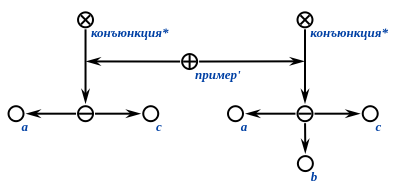
\includegraphics[scale=1.0]{./figures/sd_logic/conjunction.png}
	\end{figure}
\end{frame}

\begin{frame}{\\Дизъюнкция}
	\topline
	\justifying
	\small{
		\begin{SCn}
			\scnheader{дизъюнкция*}
			\scnidtf{логическое или*}
			\scnidtf{логическое сложение*}
			\scnidtf{включающее или*}
			\scnsubset{логическая связка*}
			\scniselement{неориентированное отношение}
			\scniselement{класс связок разной мощности}
			\scnrelfrom{пояснение}{
				\textbf{\textit{дизъюнкция*}} -- это множество дизъюнктивных \textit{высказываний}, каждое из которых истинно в рамках некоторой \textit{формальной теории} только в том случае, когда хотя бы один его компонент является истинным в рамках этой же \textit{формальной теории}.
			}
		\end{SCn}
	}
\end{frame}

\begin{frame}{\\Дизъюнкция}
	\topline
	\justifying
	\vspace{10mm}
	\begin{figure}[H]
		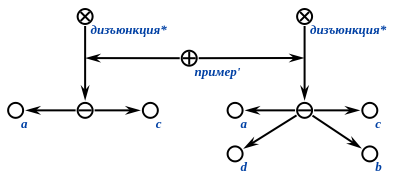
\includegraphics[scale=1.0]{./figures/sd_logic/disjunction.png}
	\end{figure}
\end{frame}

\begin{frame}{\\Отрицание}
	\topline
	\justifying
	\begin{SCn}
		\scnheader{отрицание*}
		\scnsubset{логическая связка*}
		\scnsubset{синглетон}
		\scnrelfrom{пояснение}{
			\textbf{\textit{отрицание*}} -- это множество \textit{высказываний} об отрицании, каждое из которых истинно в рамках некоторой \textit{формальной теории} только в том случае, когда его единственный элемент является ложным в рамках этой же \textit{формальной теории}.
		}
	\end{SCn}
\end{frame}

\begin{frame}{\\Отрицание}
	\topline
	\justifying
	\vspace{10mm}
	\begin{figure}[H]
		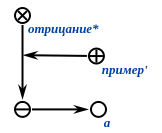
\includegraphics[scale=1.0]{./figures/sd_logic/negation.png}
	\end{figure}	
\end{frame}

\begin{frame}{\\Строгая дизъюнкция}
	\topline
	\justifying
	\begin{SCn}
		\scnheader{строгая дизъюнкция*}
		\scnidtf{сложение по модулю 2*}
		\scnidtf{исключающее или*}
		\scnidtf{альтернатива*}
		\scnsubset{логическая связка*}
		\scniselement{неориентированное отношение}
		\scniselement{класс связок разной мощности}
		\scnrelfrom{пояснение}{
			\textbf{\textit{строгая дизъюнкция*}} -- это множество строго дизъюнктивных \textit{высказываний}, каждое из которых истинно в рамках некоторой \textit{формальной теории} только в том случае, когда ровно один его компонент является истинным в рамках этой же \textit{формальной теории}.
		}
	\end{SCn}
\end{frame}

\begin{frame}{\\Строгая дизъюнкция}
	\topline
	\justifying
	\vspace{10mm}
	\begin{figure}[H]
		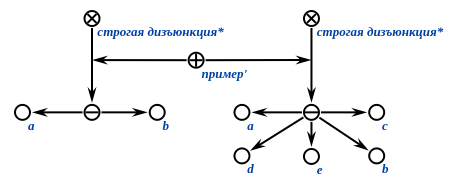
\includegraphics[scale=1.0]{./figures/sd_logic/strictDisjunction.png}
	\end{figure}	
\end{frame}

\begin{frame}{\\Импиликация}
	\topline
	\justifying
	\footnotesize{
		\begin{SCn}
			\scnheader{импликация*}
			\scnidtf{логическое следование*}
			\scnsubset{логическая связка*}
			\scniselement{бинарное отношение}
			\scniselement{ориентированное отношение}
			\scnrelfrom{пояснение}{
				\textbf{\textit{импликация*}} -- это множество импликативных \textit{неатомарных высказываний}, каждое из которых состоит из посылки (первый компонент \textit{высказывания}) и следствия (второй компонент \textit{высказывания}).
				Каждое импликативное \textit{высказывание} ложно в рамках некоторой \textit{формальной теории} в том случае, когда его посылка истинна, а заключение ложно в рамках этой же \textit{формальной теории}. В других случаях такое \textit{высказывание} истинно.
				По умолчанию на все переменные, входящие в обе части высказывания об \textbf{\textit{импликации*}} (или хотя бы одну из \textit{подформул*} каждой части) неявно накладывается квантор \textit{всеобщности*}, при условии, что эти переменные не связаны другим \textit{квантором}, указанным явно.
			}
		\end{SCn}
	}
\end{frame}

\begin{frame}{\\Импликация}
	\topline
	\justifying
	\vspace{10mm}
	\begin{figure}[H]
		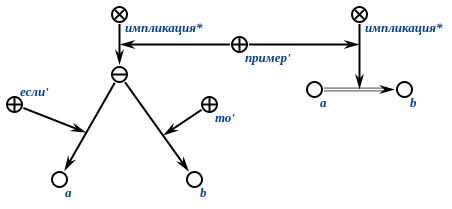
\includegraphics[scale=1.0]{./figures/sd_logic/implication.png}
	\end{figure}	
\end{frame}

\begin{frame}{\\Эквиваленция}
	\topline
	\justifying
	\footnotesize{
		\begin{SCn}
			\scnheader{эквиваленция*}
			\scnidtf{эквивалентность*}
			\scnsubset{логическая связка*}
			\scniselement{бинарное отношение}
			\scniselement{неориентированное отношение}
			\scnrelfrom{пояснение}{
				\textbf{\textit{эквиваленция*}} -- это множество \textit{высказываний} об эквивалентности, каждое из которых истинно в рамках некоторой \textit{формальной теории} только в тех случаях, когда оба его компонента одновременно либо истинны в рамках этой же \textit{формальной теории}, либо ложны.
				По умолчанию на все переменные, входящие в обе части высказывания об \textbf{\textit{эквиваленции*}} (или хотя бы одну из \textit{подформул*} каждой части) неявно накладывается квантор \textit{всеобщности*}, при условии, что эти переменные не связаны другим \textit{квантором}, указанным явно.
			}
		\end{SCn}
	}
\end{frame}

\begin{frame}{\\Эквиваленция}
	\topline
	\justifying
	\vspace{10mm}
	\begin{figure}[H]
		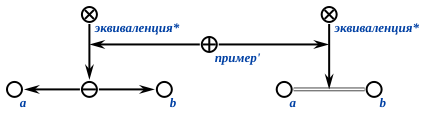
\includegraphics[scale=1.0]{./figures/sd_logic/equivalent.png}
	\end{figure}	
\end{frame}

\begin{frame}{\\ \small{Таблицы истинности логических функций}}
	\topline
	\justifying
	\vspace{5mm}
	\begin{center}
		\begin{tabular}{|c|c|c|c|c|c|c|c|}
			\hline
			$X$ & $Y$ & $\neg X$ & $X \land Y$ & $X \lor Y$ & $X \oplus Y$ & $X \to Y$ & $X \leftrightarrow Y$\\
			\hline
			$0$ & $0$ & $1$ & $0$ & $0$ & $0$ & $1$ & $1$\\
			\hline
			$0$ & $1$ & $1$ & $0$ & $1$ & $1$ & $1$ & $0$\\
			\hline
			$1$ & $0$ & $0$ & $0$ & $1$ & $1$ & $0$ & $0$\\
			\hline
			$1$ & $1$ & $0$ & $1$ & $1$ & $0$ & $1$ & $1$\\
			\hline
		\end{tabular}
	\end{center}
\end{frame}

\begin{frame}{\\Высказывание}
	\topline
	\justifying
	\begin{SCn}
			\scnheader{высказывание}
		\scnrelfrom{пояснение}{
			Под \textbf{\textit{высказыванием}} понимается некоторая \textit{структура} (в которую входят \textit{sc-константы} из некоторой предметной области и/или \textit{sc-переменные}) или \textit{логическая связка}, которая может трактоваться как истинная или ложная в рамках какой-либо \textit{предметной области}.			
		}
		\begin{scnreltoset}{\textit{разбиение}}
			\scnitem{атомарное высказывание}
			\scnitem{неатомарное высказывание}
		\end{scnreltoset}
		\begin{scnreltoset}{\textit{разбиение}}
			\scnitem{фактографическое высказывание}
			\scnitem{логическая формула}
		\end{scnreltoset}
	\end{SCn}
\end{frame}

\begin{frame}{\\Высказывание}
	\topline
	\justifying
	\\	
	Истинность \textbf{\textit{высказывания}} задается путем указания принадлежности знака этого высказывания \textit{формальной теории}, соответствующей данной \textit{предметной области}. Ложность высказывания задается путем указания принадлежности знака \textit{отрицания*} этого высказывания данной \textit{формальной теории}.\\
	Явно указанная непринадлежность \textbf{\textit{высказывания}} \textit{формальной теории} может говорить как о его ложности в рамках данной теории (если это указано рассмотренным выше образом), так и о том, что данное  \textbf{\textit{высказывание}} вообще не рассматривается в данной \textit{формальной теории} (например, использует понятия, не принадлежащие данной \textit{предметной области}).\\
	Одно и то же \textbf{\textit{высказывание}} может быть истинно в рамках одной \textit{формальной теории} и ложно в рамках другой.
\end{frame}

\begin{frame}{\\Высказывание формальной теории}
	\topline
	\justifying
	\begin{SCn}
		\scnheader{высказывание формальной теории\scnrolesign}
		\scniselement{неосновное понятие}
		\begin{scnreltoset}{разбиение}
			\scnitem{истинное высказывание\scnrolesign}			
			\scnitem{ложное высказывание\scnrolesign}			
			\scnitem{нечеткое высказывание\scnrolesign}			
			\scnitem{бессмысленное высказывание\scnrolesign}			
		\end{scnreltoset}
	\end{SCn}	
\end{frame}

\begin{frame}{\\ \small{Истинное высказывание. Ложное высказывание.}}
	\topline
	\justifying	
	\begin{SCn}
		\scnheader{истинное высказывание\scnrolesign}
		\scnidtf{высказывание, истинное в рамках данной формальной теории\scnrolesign}
		\scnidtf{высказывание, знак которого принадлежит данной формальной теории\scnrolesign}
		\scnheader{ложное высказывание\scnrolesign}
		\scnidtf{высказывание, ложное в рамках данной формальной теории\scnrolesign}
		\scnidtf{высказывание, знак отрицания которого принадлежит данной формальной теории\scnrolesign}		
	\end{SCn}	
\end{frame}

\begin{frame}{\\ \small{Нечёткое высказывание. Бессмысленное высказывание}}
	\topline
	\justifying
	\begin{SCn}
		\small{
			\scnheader{нечеткое высказывание\scnrolesign}
			\scnidtf{гипотетическое высказывание\scnrolesign}
			\scnidtf{высказывание, возможно истинное или ложное в рамках данной формальной теории\scnrolesign}
			\scnidtf{высказывание, истинное или ложное в рамках данной формальной теории с некоторой вероятностью\scnrolesign}
			\scnheader{бессмысленное высказывание\scnrolesign}
			\scnidtf{высказывание, бессмысленное в рамках данной формальной теории\scnrolesign}
			\scnidtf{высказывание, не рассматриваемое в рамках данной формальной теории\scnrolesign}
			\scnrelfrom{пояснение}{
				Высказывание является бессмысленным в рамках заданной формальной теории, если в какое-либо \textit{атомарное высказывание} в его составе (или в само это высказывание, если оно является атомарным) входит какая-либо \textit{sc-константа}, не являющаяся элементом предметной области, описываемой указанной \textit{формальной теорией}.			
			}
		}
	\end{SCn}
\end{frame}

\begin{frame}{\\ \small{Атомарное высказывание. Неатомарное высказывание}}
	\topline
	\justifying
	\footnotesize{
		\begin{SCn}
			\scnheader{атомарное высказывание}
			\scnsubset{структура}
			\begin{scnreltoset}{разбиение}
				\scnitem{атомарное фактографическое высказывание}			
				\scnitem{атомарная логическая формула}						
			\end{scnreltoset}
			\scnrelfrom{пояснение}{
				\textbf{\textit{атомарное высказывание}} -- это \textit{высказывание}, которое содержит хотя бы один \textit{sc-элемент}, не являющийся знаком другого \textit{высказывания}.
			}
			\scnheader{неатомарное высказывание}
			\scnrelfrom{пояснение}{
				\textbf{\textit{неатомарное высказывание}} -- это \textit{высказывание}, в состав которого входят только знаки других \textit{высказываний}.
				Следует отметить, что мы не можем говорить об истинности либо ложности \textbf{\textit{неатомарного высказывания}} в рамках какой-либо \textit{формальной теории}, в случае, когда невозможно установить истинность либо ложность любого из его элементов в рамках этой же \textit{формальной теории}.
			}			
		\end{SCn}
	}
\end{frame}

\begin{frame}{\\Фактографическое высказывание}
	\topline
	\justifying
	\begin{SCn}
		\scnheader{фактографическое высказывание}
		\scnsuperset{атомарное фактографическое высказывание}
		Под \textbf{фактографическим высказыванием} понимается:
		\begin{textitemize}
			\item{\textit{атомарное высказывание}, в состав которого не входит ни одна \textit{sc-переменная}}
			\item{\textit{неатомарное высказывание}, все элементы которого также являются \textbf{\textit{фактографическими высказываниями}}}
		\end{textitemize}
	\end{SCn}
\end{frame}

\begin{frame}{\\Логическая формула}
	\topline
	\justifying	
	\begin{SCn}
		\footnotesize{
			Под \textbf{логической формулой} понимается:
			\begin{textitemize}
				\item{\textit{атомарное высказывание}, в состав которого входит хотя бы одна \textit{sc-переменная};}
				\item{\textit{неатомарное высказывание}, хотя бы один элемент которого является \textbf{\textit{логической формулой}}.}
			\end{textitemize}		
			\scnheader{логическая формула}
			\begin{scnreltoset}{разбиение}
				\scnitem{атомарная логическая формула}			
				\scnitem{неатомарная логическая формула}						
			\end{scnreltoset}
			\begin{scnreltoset}{разбиение}
				\scnitem{открытая логическая формула}			
				\scnitem{замкнутая логическая формула}						
			\end{scnreltoset}
		}
	\end{SCn}
\end{frame}

\begin{frame}{\\Равносильность логических формул}
	\topline
	\justifying
	\\
	\footnotesize{
		Две формулы логики $A$ и $B$ называются равносильными, если они принимают одинаковые логические значения при любом наборе значений входящих в формулы элементарных высказываний (переменных).\\
		\textit{Обозначение}: $A \iff B$
		\begin{center}
			\begin{tabular}{|c|c|}
				\hline
				$X \land X \iff X$ & $X \lor X \iff X$\\
				\hline
				$X \land \top \iff X$ & $X \lor \top \iff \top$\\
				\hline
				$X \land \bot \iff \bot$ & $X \lor \bot \iff X$\\
				\hline
				$X \land \neg X \iff \bot$ & $X \lor \neg X \iff \top$\\
				\hline
				$\neg(\neg X) \iff X$ & $X \lor (Y \land X) \iff X$\\
				\hline
				$X \land (Y \lor X) \iff X$ & $X \leftrightarrow Y \iff (X \leftarrow Y) \land (Y \leftarrow X)$\\
				\hline
				$X \leftarrow Y \iff \neg X \lor Y$ & $\neg(X \land Y) \iff \neg X \lor \neg Y$\\
				\hline
				$\neg(X \lor Y) \iff \neg X \land \neg Y$ & $X \land Y \iff \neg(\neg X \lor \neg Y)$\\
				\hline
				$X \lor Y \iff \neg(\neg X \land \neg Y)$ &\\
				\hline
			\end{tabular}
		\end{center}
	}
\end{frame}

\begin{frame}{\\Тавтология}
	\topline
	\justifying
	\begin{SCn}
		\scnheader{тавтология}
		\scnrelfrom{пояснение}{
			\textbf{\textit{тавтология}} -- это \textit{логическая формула}, которая является либо только истинной, либо только ложной в рамках всех \textit{формальных теорий}, в которых можно установить ее истинность или ложность.\\
			\textbf{\textit{тавтология}} -- это такая \textit{логическая формула}, которая является либо \textit{общезначимой логической формулой}, либо \textit{противоречивой логической формулой}.
		}
	\end{SCn}
\end{frame}

\begin{frame}{\\Общезначимая логическая формула}
	\topline
	\justifying
	\begin{SCn}
		\scnheader{общезначимая логическая формула}
		\scnidtf{тождественно истинная логическая формула}
		\scnsubset{выполнимая логическая формула}
		\scnsubset{тавтология}
		\scnrelfrom{пояснение}{
			\textbf{\textit{общезначимая логическая формула}} -- это \textit{логическая формула}, для которой не существует \textit{формальной теории}, в рамках которой она была бы ложной с учетом истинности и ложности всех ее \textit{подформул*} в рамках этой же \textit{формальной теории}.
		}
	\end{SCn}
\end{frame}

\begin{frame}{\\Общезначимая логическая формула}
	\topline
	\justifying
	\vspace{10mm}
	\begin{figure}[H]
		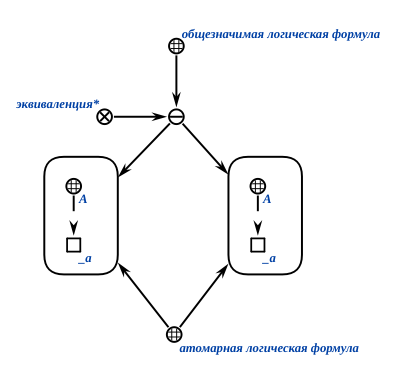
\includegraphics[scale=0.65]{./figures/sd_logic/valid_formula.png}
	\end{figure}	
\end{frame}

\begin{frame}{\\Противоречивая логическая формула}
	\topline
	\justifying
	\begin{SCn}
		\scnheader{противоречивая логическая формула}
		\scnidtf{тождественно ложная логическая формула}
		\scnsubset{невыполнимая логическая формула}
		\scnsubset{тавтология}
		\scnrelfrom{пояснение}{
			\textbf{\textit{противоречивая логическая формула}} -- это \textit{логическая формула}, для которой не существует \textit{формальной теории}, в рамках которой она была бы истинной с учетом истинности и ложности всех ее \textit{подформул*} в рамках этой же \textit{формальной теории}.
		}
	\end{SCn}
\end{frame}

\begin{frame}{\\Противоречивая логическая формула}
	\topline
	\justifying
	\vspace{10mm}
	\begin{figure}[H]
		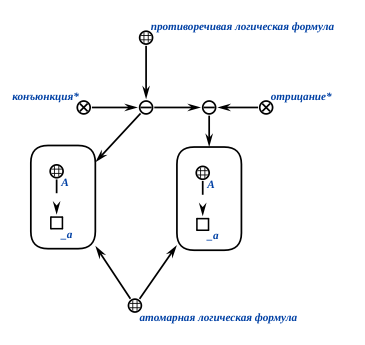
\includegraphics[scale=0.65]{./figures/sd_logic/contradiction_formula.png}
	\end{figure}	
\end{frame}

\begin{frame}{\\Нейтральная логическая формула}
	\topline
	\justifying
	\begin{SCn}
		\scnheader{нейтральная логическая формула}
		\scnsubset{выполнимая логическая формула}
		\scnrelfrom{пояснение}{
			\textbf{\textit{нейтральная логическая формула}} -- это \textit{логическая формула}, для которой существует хотя бы одна \textit{формальная теория}, в рамках которой эта формула ложна, и хотя бы одна \textit{формальная теория}, в рамках которой эта формула истинна.
		}
	\end{SCn}
\end{frame}

\begin{frame}{\\Нейтральная логическая формула}
	\topline
	\justifying
	\vspace{10mm}
	\begin{figure}[H]
		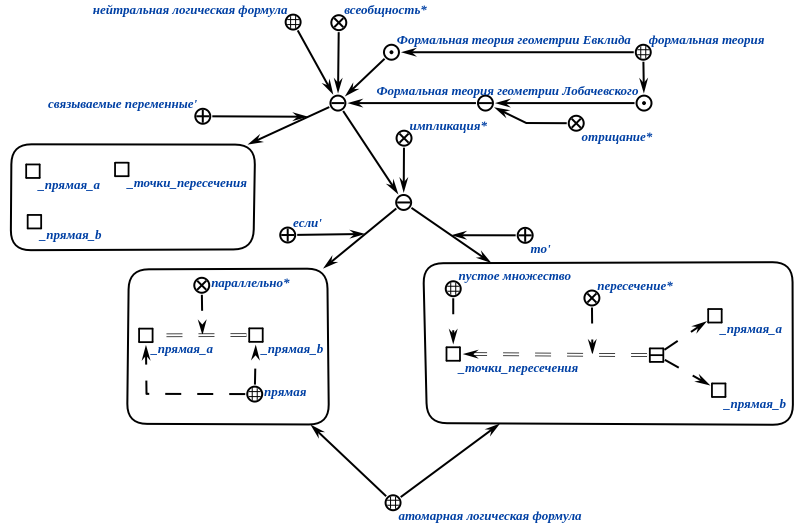
\includegraphics[scale=0.45]{./figures/sd_logic/neutral_formula.png}
	\end{figure}	
\end{frame}

\begin{frame}{\\Непротиворечивая логическая формула}
	\topline
	\justifying
	\begin{SCn}
		\scnheader{непротиворечивая логическая формула}
		\scnidtf{выполнимая логическая формула}
		\scnrelfrom{пояснение}{
			\textbf{\textit{непротиворечивая логическая формула}} -- это \textit{логическая формула}, для которой существует хотя бы одна \textit{формальная теория}, в рамках которой эта формула истинна.
		}
		\begin{scnreltoset}{объединение}
			\scnitem{нейтральная логическая формула}
			\scnitem{общезначимая логическая формула}
		\end{scnreltoset}	
	\end{SCn}
\end{frame}

\begin{frame}{\\Необщезначная логическая формула}
	\topline
	\justifying
	\begin{SCn}
		\scnheader{необщезначимая логическая формула}
		\scnidtf{невыполнимая логическая формула}
		\scnrelfrom{пояснение}{
			\textbf{\textit{необщезначимая логическая формула}} -- это \textit{логическая формула}, для которой существует хотя бы одна \textit{формальная теория}, в рамках которой эта формула ложна.
		}
		\begin{scnreltoset}{объединение}
			\scnitem{нейтральная логическая формула}
			\scnitem{противоречивая логическая формула}
		\end{scnreltoset}
	\end{SCn}
\end{frame}

\begin{frame}{\\Квантор}
	\topline
	\justifying
	\begin{SCn}
		\scnheader{квантор}
		\scnsubset{логическая связка*}
		\scnrelfrom{пояснение}{
			\textbf{\textit{квантор}} — это \textit{отношение}, каждая связка которой задает истинность множества \textit{логических формул}, входящих в ее состав, при выполнении дополнительных условий, связанных с некоторыми из переменных, входящих в состав этих \textit{логических формул}.\\
			Будем говорить, что переменные связаны \textbf{\textit{квантором}} или попадают под область действия данного \textbf{\textit{квантора}} (имея в виду конкретную связку конкретного \textbf{\textit{квантора}}).\\
			В состав каждой связки каждого \textbf{\textit{квантора}} входит \textit{атомарная формула}, являющаяся \textit{тривиальной структурой}, в которой перечислены переменные, связанные данным \textbf{\textit{квантором}}.
		}
	\end{SCn}
\end{frame}

\begin{frame}{\\Квантор всеобщности}
	\topline
	\justifying
	\footnotesize{
		\begin{SCn}
			\scnheader{всеобщность*}
			\scnidtf{квантор всеобщности*}
			\scnidtf{квантор общности*}
			\scniselement{квантор}
			\scniselement{ориентированное отношение}
			\scniselement{класс связок разной мощности}
			\scnrelfrom{пояснение}{
				\textbf{\textit{всеобщность}} -- это \textit{квантор}, для каждой связки которого, истинной в рамках некоторой \textit{формальной теории}, выполняется следующее утверждение: все формулы, входящие в состав этой связки истинны в рамках этой же \textit{формальной теории} при всех (любых) возможных значениях всех элементов множества \textit{связываемых переменных\scnrolesign} входящего в эту связку.\\
				Каждая связка \textit{квантора} \textbf{\textit{всеобщность*}} может быть представлена как \textit{конъюнкция*} (потенциально бесконечная) исходных \textit{логических формул}, входящих в состав этой связки, в каждой из которых все \textit{связанные переменные\scnrolesign} заменены на их возможные значения.
				Квантор \textbf{\textit{всеобщности*}} зачастую обозначается "$\forall$" \ и читается как "для всех"{}, "для каждого"{}, "для любого"{} или "все"{}, "каждый"{}, "любой".
			}
		\end{SCn}
	}
\end{frame}

\begin{frame}{\\Квантор всеобщности}
	\topline
	\justifying
	\vspace{10mm}
	\begin{figure}[H]
		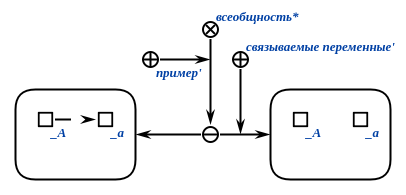
\includegraphics[scale=1.0]{./figures/sd_logic/universality.png}
	\end{figure}	
\end{frame}

\begin{frame}{\\Квантор существования}
	\topline
	\justifying
	\begin{SCn}
		\scnheader{формула существования}
		\scnidtf{существование*}
		\begin{scnreltoset}{разбиение}
			\scnitem{атомарная логическая формула}
			\scnitem{неатомарное существование*}
		\end{scnreltoset}
	\end{SCn}
\end{frame}

\begin{frame}{\\Неатомарное существование}
	\topline
	\justifying
	\footnotesize{
		\begin{SCn}
			\scnheader{неатомарное существование*}
			\scnidtf{квантор неатомарного существования*}
			\scniselement{квантор}
			\scniselement{ориентированное отношение}
			\scniselement{класс связок разной мощности}
			\scnrelfrom{пояснение}{
				\textbf{\textit{неатомарное существование*}} -- это \textit{квантор}, для каждой связки которого, истинной в рамках некоторой \textit{формальной теории}, выполняется следующее утверждение: существуют значения всех элементов множества \textit{связываемых переменных\scnrolesign} входящего в эту связку, такие, что все формулы, входящие в состав этой связки истинны в рамках этой же \textit{формальной теории}.\\
				Каждая связка \textit{квантора} \textbf{\textit{неатомарное существование*}} может быть представлена как \textit{дизъюнкция*} (потенциально бесконечная) исходных \textit{логических формул}, входящих в состав этой связки, в каждой из которых все \textit{связанные переменные\scnrolesign} заменены на их возможные значения.
				Квантор \textbf{\textit{существования*}} зачастую обозначается "$\exists$" \ и читается как "существует"{}, "для некоторого"{}, "найдется".
			}
		\end{SCn}
	}
\end{frame}

\begin{frame}{\\Неатомарное существование}
	\topline
	\justifying
	\vspace{10mm}
	\begin{figure}[H]
		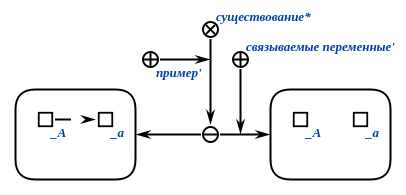
\includegraphics[scale=1.0]{./figures/sd_logic/non_atomicExistence.png}
	\end{figure}	
\end{frame}

\begin{frame}{\\Единственное существование}
	\topline
	\justifying
	\begin{SCn}
		\scnheader{единственное существование}
		\scnidtf{однократное существование}
		\scnidtf{формула существования и единственности}
		\scnrelfrom{пояснение}{
			\textbf{\textit{единственное существование}} зачастую обозначается "$\exists!$" \ и читается как "существует и единственный".
		}
	\end{SCn}
\end{frame}

\begin{frame}{\\Единственное существование}
	\topline
	\justifying
	\begin{SCn}
		\scnheader{логическая формула и единственность}
		\scnsubset{логическая формула}
		\scnsubset{единственное существование}
		\scnrelfrom{пояснение}{
			Каждый элемент множества \textbf{\textit{логическая формула и единственность}} представляет собой \textit{логическую формулу} (\textit{атомарную} или \textit{неатомарную}), для которой дополнительно уточняется, что при ее интерпретации на некоторой предметной области существует только один набор значений переменных, входящих в эту формулу (или ее \textit{подформулы*}), при котором указанная логическая формула истинна в рамках \textit{формальной теории}, в которую входит данная \textit{предметная область}.
		}
	\end{SCn}
\end{frame}

\begin{frame}{\\Единственное существование}
	\topline
	\justifying
	\vspace{10mm}
	\begin{figure}[H]
		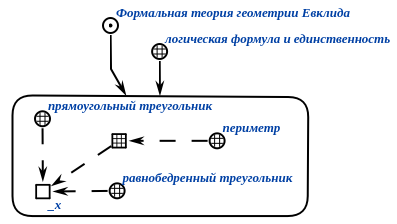
\includegraphics[scale=1.0]{./figures/sd_logic/unique_existance.png}
	\end{figure}	
\end{frame}

\begin{frame}{\\Двойственность кванторов}
	\topline
	\justifying
	\textbf{Двойственность} -- содержательное понятие, применяемое в логике и математике всякий раз, когда между двумя группами понятий установлено взаимно-однозначное соответствие так, что замена понятий одной группы на соответствующие понятия др. группы каждый раз переводит истинные высказывания в истинные высказывания.\\
	Двойственность кванторов:
	\begin{center}
		$\neg(\forall xA(x)) \iff \exists x(\neg A(x))$\\
		$\neg(\exists xA(x)) \iff \forall x(\neg A(x))$
	\end{center}
\end{frame}

\begin{frame}{\\Связываемые переменные}
	\topline
	\justifying
	\footnotesize{
		\begin{SCn}
			\scnheader{связываемые переменные\scnrolesign}
			\scniselement{ролевое отношение}
			\scnrelfrom{пояснение}{
				\textbf{\textit{связываемые переменные\scnrolesign}} -- это \textit{ролевое отношение}, которое связывает связку конкретного \textit{квантора} с множеством переменных, которые связаны этим квантором.
			}
			\scnheader{открытая логическая формула}
			\scnrelfrom{пояснение}{
				\textbf{\textit{открытая логическая формула}} -- это \textit{логическая формула}, в рамках которой (и всех ее \textit{подформул*}) существует хотя бы одна переменная, не связанная никаким \textit{квантором}.
			}
			\scnheader{замкнутая логическая формула}
			\scnrelfrom{пояснение}{
				\textbf{\textit{замкнутая логическая формула}} -- это \textit{логическая формула}, в рамках которой (и всех ее \textit{подформул*}) не существует переменных, не связанных каким-либо \textit{квантором}.
			}
		\end{SCn}
	}
\end{frame}
